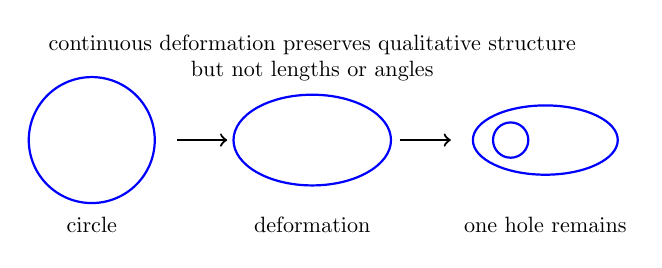
\begin{tikzpicture}[scale=.8,transform shape]
\draw[thick,blue] (0,0) circle (1);
\node at (0,-1.35) {circle};
\draw[thick,->] (1.35,0)--(2.15,0);
\draw[thick,blue] (3.5,0) ellipse (1.25 and .72);
\node at (3.5,-1.35) {deformation};
\draw[thick,->] (4.9,0)--(5.7,0);
\draw[thick,blue] (7.2,0) ellipse (1.15 and .55);
\draw[thick,blue] (6.65,0) circle (.28);
\node at (7.2,-1.35) {one hole remains};
\node[align=center] at (3.5,1.3) {continuous deformation preserves qualitative structure\\but not lengths or angles};
\end{tikzpicture}
